\documentclass[
	a4paper, % Paper size, use either a4paper or letterpaper
	10pt, % Default font size, can also use 11pt or 12pt, although this is not recommended
	unnumberedsections, % Comment to enable section numbering
	twoside, % Two side traditional mode where headers and footers change between odd and even pages, comment this option to make them fixed
]{LTJournalArticle}


\usepackage[]{amsmath}
\usepackage{graphicx}
\usepackage{tikz} 
\usetikzlibrary{calc}
\addbibresource{sample.bib} % BibLaTeX bibliography file

% A shortened article title to appear in the running head, leave this command empty for no running head

% \footertext{\textit{Journal of Biological Sampling} (2024) 12:533-684} % Text to appear in the footer, leave this command empty for no footer text

\setcounter{page}{1} % The page number of the first page, set this to a higher number if the article is to be part of an issue or larger work

%----------------------------------------------------------------------------------------
%	TITLE SECTION
%----------------------------------------------------------------------------------------

\title{CS262 Design Excercise Three \\ Replication} % Article title, use manual lines breaks (\\) to beautify the layout

% Authors are listed in a comma-separated list with superscript numbers indicating affiliations
% \thanks{} is used for any text that should be placed in a footnote on the first page, such as the corresponding author's email, journal acceptance dates, a copyright/license notice, keywords, etc
\author{%
	Swati Goel and Artemas Radik
}


%----------------------------------------------------------------------------------------

\begin{document}

\maketitle % Output the title section

%----------------------------------------------------------------------------------------
%	ARTICLE CONTENTS
%----------------------------------------------------------------------------------------

\section{I. Introduction}

We considered several approaches for implementation, including (but not limited to) the PAXOS algorithm as well as traditional Primary/Secondary Replication. However, all of these approaches were rather overcomplicated for the problem at hand.

\smallskip
We see our new approach as a much better solution to the design exercise for several reasons. Firstly, It's significantly easier to implement than any other approach and requires minimal modification to our existing codebase from design excercise one.

\smallskip
Furthermore, it's not relevant here for the servers to have a synchronized global state, as messages are only exchanged between two users. Thus, it's simply important for these two users to agree on the message exchange order between themselves. 

\smallskip
A way we thought about this was considering Apple's iMessage: it does not care about whether a message sent between two US users was sent before or after a message sent between two EU users (ie, ordering irrelevant). It simply cares that the ordering of messages on both endpoint devices, in each conversation, is consistent.


\section{II. Edge Cases}
In our system design, several edge cases arose for which we needed to account for.
\begin{enumerate}
	\item Storing received-yet-unsent messages on-disk is not sufficient for server persistence. Imagine the case where a message is sent by a client and received by the server (so TCP succeeds and does not retransmit) but then the server dies before buffering the message and saving it on-disk. Hence any messages sitting in the server's socket stream are also not persisted upon failure.
	\item What happens when the entire distributed system is brough offline, some time passes, and then it's brought back online? How do we handle data that is potentially in network transit at the time of system death?
	\item How do we prevent repeated retransmission of identical data, which would be both slow and expensive at large scales?
\end{enumerate}

\section{III. Our Approach}

We propose a multicast architecture where replication is handled independently. Consider the graph below, which models our message upload architecture. When a client $c_1$ wishes to send a message $m$ to client $c_2$, three uploads $u_1,u_2,u_3$ containing $m$ are initiated. These uploads are made asynchronously to servers $s_1,s_2,s_3$. Each server then proceeds to return $a_1,a_2,a_3$ to $c_1$, acknowledging receipt of the uploads.

\begin{figure}[!h]
	\centering
	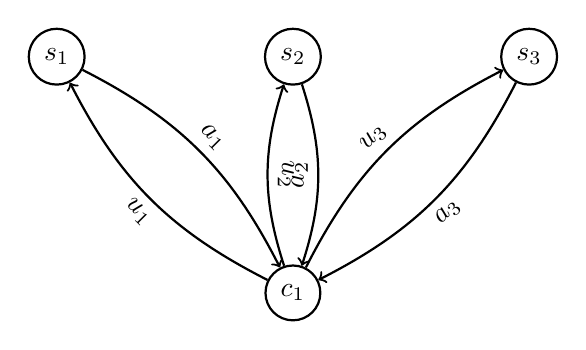
\begin{tikzpicture}[node distance={30mm}, thick, main/.style = {draw, circle}] 
		\node[main] (1) {$s_1$}; 
		\node[main] (2) [right of=1] {$s_2$}; 
		\node[main] (3) [right of=2] {$s_3$}; 
		\node[main] (4) [below of=2] {$c_1$}; 
		\draw[->] (4) to [bend left=18] node[midway, sloped, below] {$u_1$} (1);
		\draw[->] (1) to [bend left=18] node[midway, sloped, above] {$a_1$} (4);
		\draw[->] (4) to [bend left=18] node[midway, sloped, above] {$u_2$} (2);
		\draw[->] (2) to [bend left=18] node[midway, sloped, above] {$a_2$} (4);
		\draw[->] (4) to [bend left=18] node[midway, sloped, above] {$u_3$} (3);
		\draw[->] (3) to [bend left=18] node[midway, sloped, below] {$a_3$} (4);
	\end{tikzpicture} 
\end{figure}

We note that this system is two-fault tolerant, since $c_1$ only reports to its user that it has successfully sent a requested message once $c_1$ receives acknowledgements from all online servers. If only two out of three online servers acknowledge receipt, we cannot guarantee safety, as it is possible for both servers to fail immediately after dispersing their acknowledgements but before delivering the message to the end recipient. We note that once a server is known to be offline, we can ignore its acknowledgements, as we count it towards the two-fault tolerant requirement.

\smallskip
This system is also persistent, as the servers only deliver acknowledgements as soon as they have persisted data to disk. Furthermore, the entire system can shut down at any point and and data loss is mitigated. If the entire system reboots:

\begin{enumerate}
	\item while an acknowledgement is in transit, the client detects that an acknowledgement was never received, so it retries sending the message. The server then detects a the message as a duplicate and resends the acknowledgement, completing the cycle.
	\item while an upload is in transit, the client detects a lack of acknowledgement and hence resends the upload, restarting the cycle.
\end{enumerate}

We further note that the synchronous dispatch ordering of messages to servers enforces ordering as an invariant. Consider the scenario where client A sends "Hello" and then "World". Although one server (lets say it's in Alaska and has bad internet) may receive "Hello" after another server already receives "World", it does not matter because any server that has received "World" must have already received "Hello", as the client dispatches messages sequentially and synchronously on a per-server basis.

\smallskip
We mirror the upload process with a similar delivery system, where $d_4,d_5,d_6$ represent deliveries of the message to $c_2$ with acknowledgements $a_4, a_5, a_6$.
\begin{figure}[!h]
	\centering
	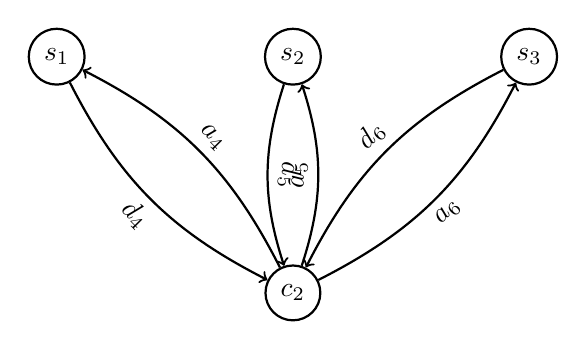
\begin{tikzpicture}[node distance={30mm}, thick, main/.style = {draw, circle}] 
		\node[main] (1) {$s_1$}; 
		\node[main] (2) [right of=1] {$s_2$}; 
		\node[main] (3) [right of=2] {$s_3$}; 
		\node[main] (4) [below of=2] {$c_2$}; 
		\draw[<-] (4) to [bend left=18] node[midway, sloped, below] {$d_4$} (1);
		\draw[<-] (1) to [bend left=18] node[midway, sloped, above] {$a_4$} (4);
		\draw[<-] (4) to [bend left=18] node[midway, sloped, above] {$d_5$} (2);
		\draw[<-] (2) to [bend left=18] node[midway, sloped, above] {$a_5$} (4);
		\draw[<-] (4) to [bend left=18] node[midway, sloped, above] {$d_6$} (3);
		\draw[<-] (3) to [bend left=18] node[midway, sloped, below] {$a_6$} (4);
	\end{tikzpicture} 
\end{figure}

We note that the delivery  process is similarly two-fault tolerant as well as persistent due to idential (but mirrored) reasons as the upload system. Although it may be intuitive, it's worth mentioning that $c_2$ only needs to receive a message with a certain GUID once to display it, since we can trust the servers completely, as we're not accounting for Byzantine faults here.

\section{IV. Improvements}
Though these were not implemented, it would be relatively straightforward to implement several improvements to this system. To begin, we can easily make the system two-fault tolerant (and $k$-fault tolerant, but that is out of scope) for Byzantine faults. By having six servers instead of three, and requiring the client to receive a given message atleast four times before displaying it, we guarantee Byzantine safety. 

\smallskip
This is because a majority of servers have to deliver the message before it is deemed legitimate. If two servers edit the content of a given message, then its hash would change, and hence it would count as effectively a seperate message. Thus up to two servers could be malicious and yet still the client would only print legitimate messages. We note that we could implement such functionality client-side via a hash table.

\smallskip
Another significant improvement that could be made is the use of IP Multicasting. This operation, which is part of the Internet Protocol, uses multicast trees to ``allow a single transmission to branch out to the desired receivers. The branches are created at the Internet routers, the branches are created such that the length of the transmission will be minimum'' (Multicasting in Computer Network, GeeksForGeeks.org). In other words, transmissions are MSTs rather than successive traverses of the shortest available path.

\smallskip
Even though IP multicasting still requires total network bandwith that is far greater than a direct approach, we see this as a valid tradeoff to make: optimizing for simpler, less buggy code in exchange for slightly worse performance.

\end{document}
